% Options for packages loaded elsewhere
\PassOptionsToPackage{unicode}{hyperref}
\PassOptionsToPackage{hyphens}{url}
%
\documentclass[
]{article}
\usepackage{amsmath,amssymb}
\usepackage{lmodern}
\usepackage{ifxetex,ifluatex}
\ifnum 0\ifxetex 1\fi\ifluatex 1\fi=0 % if pdftex
  \usepackage[T1]{fontenc}
  \usepackage[utf8]{inputenc}
  \usepackage{textcomp} % provide euro and other symbols
\else % if luatex or xetex
  \usepackage{unicode-math}
  \defaultfontfeatures{Scale=MatchLowercase}
  \defaultfontfeatures[\rmfamily]{Ligatures=TeX,Scale=1}
\fi
% Use upquote if available, for straight quotes in verbatim environments
\IfFileExists{upquote.sty}{\usepackage{upquote}}{}
\IfFileExists{microtype.sty}{% use microtype if available
  \usepackage[]{microtype}
  \UseMicrotypeSet[protrusion]{basicmath} % disable protrusion for tt fonts
}{}
\makeatletter
\@ifundefined{KOMAClassName}{% if non-KOMA class
  \IfFileExists{parskip.sty}{%
    \usepackage{parskip}
  }{% else
    \setlength{\parindent}{0pt}
    \setlength{\parskip}{6pt plus 2pt minus 1pt}}
}{% if KOMA class
  \KOMAoptions{parskip=half}}
\makeatother
\usepackage{xcolor}
\IfFileExists{xurl.sty}{\usepackage{xurl}}{} % add URL line breaks if available
\IfFileExists{bookmark.sty}{\usepackage{bookmark}}{\usepackage{hyperref}}
\hypersetup{
  pdftitle={Discussion on 05/04/2022},
  pdfauthor={Duc Du, Thinh Ong},
  hidelinks,
  pdfcreator={LaTeX via pandoc}}
\urlstyle{same} % disable monospaced font for URLs
\usepackage[margin=1in]{geometry}
\usepackage{color}
\usepackage{fancyvrb}
\newcommand{\VerbBar}{|}
\newcommand{\VERB}{\Verb[commandchars=\\\{\}]}
\DefineVerbatimEnvironment{Highlighting}{Verbatim}{commandchars=\\\{\}}
% Add ',fontsize=\small' for more characters per line
\usepackage{framed}
\definecolor{shadecolor}{RGB}{248,248,248}
\newenvironment{Shaded}{\begin{snugshade}}{\end{snugshade}}
\newcommand{\AlertTok}[1]{\textcolor[rgb]{0.94,0.16,0.16}{#1}}
\newcommand{\AnnotationTok}[1]{\textcolor[rgb]{0.56,0.35,0.01}{\textbf{\textit{#1}}}}
\newcommand{\AttributeTok}[1]{\textcolor[rgb]{0.77,0.63,0.00}{#1}}
\newcommand{\BaseNTok}[1]{\textcolor[rgb]{0.00,0.00,0.81}{#1}}
\newcommand{\BuiltInTok}[1]{#1}
\newcommand{\CharTok}[1]{\textcolor[rgb]{0.31,0.60,0.02}{#1}}
\newcommand{\CommentTok}[1]{\textcolor[rgb]{0.56,0.35,0.01}{\textit{#1}}}
\newcommand{\CommentVarTok}[1]{\textcolor[rgb]{0.56,0.35,0.01}{\textbf{\textit{#1}}}}
\newcommand{\ConstantTok}[1]{\textcolor[rgb]{0.00,0.00,0.00}{#1}}
\newcommand{\ControlFlowTok}[1]{\textcolor[rgb]{0.13,0.29,0.53}{\textbf{#1}}}
\newcommand{\DataTypeTok}[1]{\textcolor[rgb]{0.13,0.29,0.53}{#1}}
\newcommand{\DecValTok}[1]{\textcolor[rgb]{0.00,0.00,0.81}{#1}}
\newcommand{\DocumentationTok}[1]{\textcolor[rgb]{0.56,0.35,0.01}{\textbf{\textit{#1}}}}
\newcommand{\ErrorTok}[1]{\textcolor[rgb]{0.64,0.00,0.00}{\textbf{#1}}}
\newcommand{\ExtensionTok}[1]{#1}
\newcommand{\FloatTok}[1]{\textcolor[rgb]{0.00,0.00,0.81}{#1}}
\newcommand{\FunctionTok}[1]{\textcolor[rgb]{0.00,0.00,0.00}{#1}}
\newcommand{\ImportTok}[1]{#1}
\newcommand{\InformationTok}[1]{\textcolor[rgb]{0.56,0.35,0.01}{\textbf{\textit{#1}}}}
\newcommand{\KeywordTok}[1]{\textcolor[rgb]{0.13,0.29,0.53}{\textbf{#1}}}
\newcommand{\NormalTok}[1]{#1}
\newcommand{\OperatorTok}[1]{\textcolor[rgb]{0.81,0.36,0.00}{\textbf{#1}}}
\newcommand{\OtherTok}[1]{\textcolor[rgb]{0.56,0.35,0.01}{#1}}
\newcommand{\PreprocessorTok}[1]{\textcolor[rgb]{0.56,0.35,0.01}{\textit{#1}}}
\newcommand{\RegionMarkerTok}[1]{#1}
\newcommand{\SpecialCharTok}[1]{\textcolor[rgb]{0.00,0.00,0.00}{#1}}
\newcommand{\SpecialStringTok}[1]{\textcolor[rgb]{0.31,0.60,0.02}{#1}}
\newcommand{\StringTok}[1]{\textcolor[rgb]{0.31,0.60,0.02}{#1}}
\newcommand{\VariableTok}[1]{\textcolor[rgb]{0.00,0.00,0.00}{#1}}
\newcommand{\VerbatimStringTok}[1]{\textcolor[rgb]{0.31,0.60,0.02}{#1}}
\newcommand{\WarningTok}[1]{\textcolor[rgb]{0.56,0.35,0.01}{\textbf{\textit{#1}}}}
\usepackage{graphicx}
\makeatletter
\def\maxwidth{\ifdim\Gin@nat@width>\linewidth\linewidth\else\Gin@nat@width\fi}
\def\maxheight{\ifdim\Gin@nat@height>\textheight\textheight\else\Gin@nat@height\fi}
\makeatother
% Scale images if necessary, so that they will not overflow the page
% margins by default, and it is still possible to overwrite the defaults
% using explicit options in \includegraphics[width, height, ...]{}
\setkeys{Gin}{width=\maxwidth,height=\maxheight,keepaspectratio}
% Set default figure placement to htbp
\makeatletter
\def\fps@figure{htbp}
\makeatother
\setlength{\emergencystretch}{3em} % prevent overfull lines
\providecommand{\tightlist}{%
  \setlength{\itemsep}{0pt}\setlength{\parskip}{0pt}}
\setcounter{secnumdepth}{-\maxdimen} % remove section numbering
\ifluatex
  \usepackage{selnolig}  % disable illegal ligatures
\fi

\title{Discussion on 05/04/2022}
\author{Duc Du, Thinh Ong}
\date{2022-06-03}

\begin{document}
\maketitle

{
\setcounter{tocdepth}{2}
\tableofcontents
}
\begin{Shaded}
\begin{Highlighting}[]
\NormalTok{knitr}\SpecialCharTok{::}\NormalTok{opts\_chunk}\SpecialCharTok{$}\FunctionTok{set}\NormalTok{(}\AttributeTok{warning =} \ConstantTok{FALSE}\NormalTok{, }\AttributeTok{message =} \ConstantTok{FALSE}\NormalTok{, }\AttributeTok{cache.lazy =} \ConstantTok{FALSE}\NormalTok{, }\AttributeTok{tidy.opts=}\FunctionTok{list}\NormalTok{(}\AttributeTok{width.cutoff=}\DecValTok{60}\NormalTok{), }\AttributeTok{tidy=}\ConstantTok{TRUE}\NormalTok{, }\AttributeTok{root.dir =}\NormalTok{ rprojroot}\SpecialCharTok{::}\FunctionTok{find\_rstudio\_root\_file}\NormalTok{())}

\FunctionTok{library}\NormalTok{(data.table)}
\FunctionTok{library}\NormalTok{(dplyr)}
\FunctionTok{library}\NormalTok{(tidyr)}
\FunctionTok{library}\NormalTok{(lubridate)}
\FunctionTok{library}\NormalTok{(ggplot2)}

\CommentTok{\# Path to dataset}
\NormalTok{allp }\OtherTok{\textless{}{-}} \FunctionTok{file.path}\NormalTok{(}\StringTok{"\textasciitilde{}"}\NormalTok{, }\StringTok{"updated\_dataset"}\NormalTok{)}
\CommentTok{\# Load vector of public provinces names}
\NormalTok{publicProvinces }\OtherTok{\textless{}{-}} \FunctionTok{readRDS}\NormalTok{(}\StringTok{"\textasciitilde{}/Vaccination\_COVID/data/publicProvinces.rds"}\NormalTok{)}
\end{Highlighting}
\end{Shaded}

Load and process measles dataset

\begin{Shaded}
\begin{Highlighting}[]
\CommentTok{\# Load measles data}
\FunctionTok{load}\NormalTok{(}\FunctionTok{file.path}\NormalTok{(allp, }\StringTok{"measle\_all.Rdata"}\NormalTok{))}
\CommentTok{\# Get children and public provinces only}
\NormalTok{measle\_all }\OtherTok{\textless{}{-}}\NormalTok{ measle\_all[measle\_all}\SpecialCharTok{$}\NormalTok{province }\SpecialCharTok{\%in\%}\NormalTok{ publicProvinces }\SpecialCharTok{\&}
\NormalTok{    measle\_all}\SpecialCharTok{$}\NormalTok{year }\SpecialCharTok{\textgreater{}=} \DecValTok{2017} \SpecialCharTok{\&}\NormalTok{ measle\_all}\SpecialCharTok{$}\NormalTok{year }\SpecialCharTok{\textless{}=} \DecValTok{2020}\NormalTok{, ]}
\NormalTok{measle\_all }\OtherTok{\textless{}{-}}\NormalTok{ measle\_all }\SpecialCharTok{\%\textgreater{}\%}
    \FunctionTok{distinct}\NormalTok{(., pid, province, district, commune, sex, dob, vacname2,}
\NormalTok{        vacdate, }\AttributeTok{.keep\_all =} \ConstantTok{TRUE}\NormalTok{)}
\NormalTok{measle\_all }\OtherTok{\textless{}{-}}\NormalTok{ measle\_all }\SpecialCharTok{\%\textgreater{}\%}
    \FunctionTok{group\_by}\NormalTok{(pid, vacname2) }\SpecialCharTok{\%\textgreater{}\%}
    \FunctionTok{arrange}\NormalTok{(vacdate) }\SpecialCharTok{\%\textgreater{}\%}
    \FunctionTok{mutate}\NormalTok{(}\AttributeTok{shot =} \DecValTok{1}\SpecialCharTok{:}\FunctionTok{n}\NormalTok{()) }\SpecialCharTok{\%\textgreater{}\%}
    \FunctionTok{ungroup}\NormalTok{()}
\NormalTok{measle\_all }\OtherTok{\textless{}{-}} \FunctionTok{data.table}\NormalTok{(measle\_all)}
\NormalTok{measle\_all}\SpecialCharTok{$}\NormalTok{age }\OtherTok{\textless{}{-}} \DecValTok{2021} \SpecialCharTok{{-}}\NormalTok{ measle\_all}\SpecialCharTok{$}\NormalTok{year}
\NormalTok{measle\_all}\SpecialCharTok{$}\NormalTok{sex }\OtherTok{\textless{}{-}} \FunctionTok{ifelse}\NormalTok{(measle\_all}\SpecialCharTok{$}\NormalTok{sex }\SpecialCharTok{==} \DecValTok{2}\NormalTok{, }\DecValTok{1}\NormalTok{, measle\_all}\SpecialCharTok{$}\NormalTok{sex)}
\NormalTok{measle\_all}\SpecialCharTok{$}\NormalTok{sex }\OtherTok{\textless{}{-}} \FunctionTok{factor}\NormalTok{(measle\_all}\SpecialCharTok{$}\NormalTok{sex, }\AttributeTok{levels =} \FunctionTok{c}\NormalTok{(}\DecValTok{0}\NormalTok{, }\DecValTok{1}\NormalTok{), }\AttributeTok{labels =} \FunctionTok{c}\NormalTok{(}\StringTok{"F"}\NormalTok{,}
    \StringTok{"M"}\NormalTok{))}
\NormalTok{measle\_all}\SpecialCharTok{$}\NormalTok{shot2 }\OtherTok{\textless{}{-}} \FunctionTok{ifelse}\NormalTok{(measle\_all}\SpecialCharTok{$}\NormalTok{shot }\SpecialCharTok{\textgreater{}=} \DecValTok{2}\NormalTok{, }\DecValTok{2}\NormalTok{, measle\_all}\SpecialCharTok{$}\NormalTok{shot)}
\NormalTok{measle\_all}\SpecialCharTok{$}\NormalTok{start2 }\OtherTok{\textless{}{-}} \FunctionTok{ifelse}\NormalTok{(measle\_all}\SpecialCharTok{$}\NormalTok{shot2 }\SpecialCharTok{==} \DecValTok{2}\NormalTok{, }\ConstantTok{NA}\NormalTok{, measle\_all}\SpecialCharTok{$}\NormalTok{start)}
\NormalTok{measle\_all}\SpecialCharTok{$}\NormalTok{start2 }\OtherTok{\textless{}{-}} \FunctionTok{ifelse}\NormalTok{(measle\_all}\SpecialCharTok{$}\NormalTok{vacname2 }\SpecialCharTok{==} \StringTok{"Measle\_Mumps\_Rubella"} \SpecialCharTok{\&}
\NormalTok{    measle\_all}\SpecialCharTok{$}\NormalTok{shot2 }\SpecialCharTok{==} \DecValTok{1}\NormalTok{, }\DecValTok{12}\NormalTok{, measle\_all}\SpecialCharTok{$}\NormalTok{start2)}
\NormalTok{measle\_all}\SpecialCharTok{$}\NormalTok{vdelay2 }\OtherTok{\textless{}{-}}\NormalTok{ measle\_all}\SpecialCharTok{$}\NormalTok{vagem2 }\SpecialCharTok{{-}}\NormalTok{ measle\_all}\SpecialCharTok{$}\NormalTok{start2}
\NormalTok{measle\_all }\OtherTok{\textless{}{-}}\NormalTok{ measle\_all[measle\_all}\SpecialCharTok{$}\NormalTok{shot }\SpecialCharTok{==} \DecValTok{1}\NormalTok{, ]}
\NormalTok{measle\_all}\SpecialCharTok{$}\NormalTok{expect\_vdate }\OtherTok{\textless{}{-}}\NormalTok{ measle\_all}\SpecialCharTok{$}\NormalTok{dob }\SpecialCharTok{\%m+\%} \FunctionTok{months}\NormalTok{(measle\_all}\SpecialCharTok{$}\NormalTok{start2)}
\end{Highlighting}
\end{Shaded}

\hypertarget{individual-level}{%
\subsection{Individual level}\label{individual-level}}

Extract children who get 2 shots

\begin{Shaded}
\begin{Highlighting}[]
\NormalTok{measles\_2shots }\OtherTok{\textless{}{-}}\NormalTok{ measle\_all[}\FunctionTok{duplicated}\NormalTok{(measle\_all}\SpecialCharTok{$}\NormalTok{pid) }\SpecialCharTok{|} \FunctionTok{duplicated}\NormalTok{(measle\_all}\SpecialCharTok{$}\NormalTok{pid,}
    \AttributeTok{fromLast =}\NormalTok{ T), ]}

\NormalTok{dup\_sameday }\OtherTok{\textless{}{-}}\NormalTok{ measles\_2shots[}\FunctionTok{duplicated}\NormalTok{(measles\_2shots[, }\FunctionTok{c}\NormalTok{(}\StringTok{"pid"}\NormalTok{,}
    \StringTok{"vacdate"}\NormalTok{)]) }\SpecialCharTok{|} \FunctionTok{duplicated}\NormalTok{(measles\_2shots[, }\FunctionTok{c}\NormalTok{(}\StringTok{"pid"}\NormalTok{, }\StringTok{"vacdate"}\NormalTok{)],}
    \AttributeTok{fromLast =}\NormalTok{ T), }\FunctionTok{c}\NormalTok{(}\StringTok{"pid"}\NormalTok{, }\StringTok{"vacdate"}\NormalTok{, }\StringTok{"vacname2"}\NormalTok{, }\StringTok{"type2"}\NormalTok{)]}
\FunctionTok{head}\NormalTok{(dup\_sameday, }\DecValTok{10}\NormalTok{)}
\end{Highlighting}
\end{Shaded}

\begin{verbatim}
##                 pid    vacdate             vacname2   type2
##  1: 201033720170006 2017-10-10               Measle  public
##  2: 201033720170006 2017-10-10       Measle_Rubella  public
##  3: 213092120170006 2017-10-12               Measle  public
##  4: 213092120170006 2017-10-12       Measle_Rubella  public
##  5: 101430120170024 2017-10-27               Measle  public
##  6: 101430120170024 2017-10-27 Measle_Mumps_Rubella private
##  7: 101012320170037 2017-11-01               Measle  public
##  8: 101012320170037 2017-11-01 Measle_Mumps_Rubella private
##  9: 101012320170094 2017-11-23               Measle  public
## 10: 101012320170094 2017-11-23 Measle_Mumps_Rubella private
\end{verbatim}

Some received the same vaccine in the same day, filter them out and
continue

\begin{Shaded}
\begin{Highlighting}[]
\CommentTok{\# Remove children with multiple shots of measles in the}
\CommentTok{\# same day}
\NormalTok{measles\_2shots }\OtherTok{\textless{}{-}}\NormalTok{ measles\_2shots }\SpecialCharTok{\%\textgreater{}\%}
    \FunctionTok{distinct}\NormalTok{(., pid, vacdate, }\AttributeTok{.keep\_all =}\NormalTok{ T)}

\CommentTok{\# Now subset the one still get 2 shots}
\NormalTok{measles\_2shots }\OtherTok{\textless{}{-}}\NormalTok{ measles\_2shots[}\FunctionTok{duplicated}\NormalTok{(measles\_2shots}\SpecialCharTok{$}\NormalTok{pid) }\SpecialCharTok{|}
    \FunctionTok{duplicated}\NormalTok{(measles\_2shots}\SpecialCharTok{$}\NormalTok{pid, }\AttributeTok{fromLast =}\NormalTok{ T), ]}

\CommentTok{\# Sort by vaccination date and numbering the shot}
\NormalTok{measles\_2shots }\OtherTok{\textless{}{-}}\NormalTok{ measles\_2shots }\SpecialCharTok{\%\textgreater{}\%}
    \FunctionTok{group\_by}\NormalTok{(pid) }\SpecialCharTok{\%\textgreater{}\%}
    \FunctionTok{arrange}\NormalTok{(vacdate) }\SpecialCharTok{\%\textgreater{}\%}
    \FunctionTok{mutate}\NormalTok{(}\AttributeTok{vtimes =} \DecValTok{1}\SpecialCharTok{:}\FunctionTok{n}\NormalTok{(), }\AttributeTok{vacdate\_1st =} \FunctionTok{first}\NormalTok{(vacdate)) }\SpecialCharTok{\%\textgreater{}\%}
    \FunctionTok{ungroup}\NormalTok{()}

\CommentTok{\# How many shots they receive}
\FunctionTok{table}\NormalTok{(measles\_2shots}\SpecialCharTok{$}\NormalTok{vtimes)}
\end{Highlighting}
\end{Shaded}

\begin{verbatim}
## 
##       1       2       3 
## 1622531 1622531   85123
\end{verbatim}

Some received 3 shots, filtered them out.

\begin{Shaded}
\begin{Highlighting}[]
\CommentTok{\# Remove those who get the 3rd shot}
\NormalTok{measles\_2shots }\OtherTok{\textless{}{-}}\NormalTok{ measles\_2shots[measles\_2shots}\SpecialCharTok{$}\NormalTok{vtimes }\SpecialCharTok{!=} \DecValTok{3}\NormalTok{,}
\NormalTok{    ]}
\NormalTok{measles\_2shots }\OtherTok{\textless{}{-}}\NormalTok{ measles\_2shots[}\FunctionTok{order}\NormalTok{(measles\_2shots}\SpecialCharTok{$}\NormalTok{pid), ]}

\CommentTok{\# Prefix \textquotesingle{}shot\textquotesingle{} to vtimes to make wide data frame easier}
\NormalTok{measles\_2shots}\SpecialCharTok{$}\NormalTok{vtimes }\OtherTok{\textless{}{-}} \FunctionTok{paste0}\NormalTok{(}\StringTok{"shot"}\NormalTok{, measles\_2shots}\SpecialCharTok{$}\NormalTok{vtimes)}
\end{Highlighting}
\end{Shaded}

Change dataset from long to wide format

\begin{Shaded}
\begin{Highlighting}[]
\NormalTok{df }\OtherTok{\textless{}{-}}\NormalTok{ measles\_2shots[, }\FunctionTok{c}\NormalTok{(}\StringTok{"pid"}\NormalTok{, }\StringTok{"vacdate\_1st"}\NormalTok{, }\StringTok{"vtimes"}\NormalTok{, }\StringTok{"type2"}\NormalTok{)]}
\NormalTok{df }\OtherTok{\textless{}{-}}\NormalTok{ df }\SpecialCharTok{\%\textgreater{}\%}
    \FunctionTok{pivot\_wider}\NormalTok{(., }\AttributeTok{names\_from =}\NormalTok{ vtimes, }\AttributeTok{values\_from =}\NormalTok{ type2)}

\NormalTok{df}\SpecialCharTok{$}\NormalTok{vyear\_1st }\OtherTok{\textless{}{-}} \FunctionTok{year}\NormalTok{(df}\SpecialCharTok{$}\NormalTok{vacdate\_1st)}
\NormalTok{df}\SpecialCharTok{$}\NormalTok{vmonth\_1st }\OtherTok{\textless{}{-}} \FunctionTok{month}\NormalTok{(df}\SpecialCharTok{$}\NormalTok{vacdate\_1st)}

\FunctionTok{head}\NormalTok{(df)}
\end{Highlighting}
\end{Shaded}

\begin{verbatim}
## # A tibble: 6 x 6
##   pid             vacdate_1st shot1  shot2   vyear_1st vmonth_1st
##   <chr>           <date>      <fct>  <fct>       <dbl>      <dbl>
## 1 101010120170003 2017-11-05  public public       2017         11
## 2 101010120170006 2017-11-05  public private      2017         11
## 3 101010120170007 2017-12-13  public private      2017         12
## 4 101010120170008 2017-10-05  public public       2017         10
## 5 101010120170014 2018-01-10  public public       2018          1
## 6 101010120170015 2017-11-15  public public       2017         11
\end{verbatim}

Aggregate them by month

\begin{Shaded}
\begin{Highlighting}[]
\NormalTok{df\_type }\OtherTok{\textless{}{-}} \FunctionTok{aggregate}\NormalTok{(pid }\SpecialCharTok{\textasciitilde{}}\NormalTok{ vyear\_1st }\SpecialCharTok{+}\NormalTok{ vmonth\_1st }\SpecialCharTok{+}\NormalTok{ shot1 }\SpecialCharTok{+}\NormalTok{ shot2,}
    \AttributeTok{data =}\NormalTok{ df, }\AttributeTok{FUN =}\NormalTok{ length)}

\NormalTok{df\_type }\OtherTok{\textless{}{-}}\NormalTok{ df\_type }\SpecialCharTok{\%\textgreater{}\%}
    \FunctionTok{group\_by}\NormalTok{(vyear\_1st, vmonth\_1st, shot1) }\SpecialCharTok{\%\textgreater{}\%}
    \FunctionTok{mutate}\NormalTok{(}\AttributeTok{denom =} \FunctionTok{sum}\NormalTok{(pid))}

\NormalTok{df\_type}\SpecialCharTok{$}\NormalTok{pct2 }\OtherTok{\textless{}{-}} \DecValTok{100} \SpecialCharTok{*}\NormalTok{ df\_type}\SpecialCharTok{$}\NormalTok{pid}\SpecialCharTok{/}\NormalTok{df\_type}\SpecialCharTok{$}\NormalTok{denom}

\CommentTok{\# Take 01/2018 as an example}
\NormalTok{df\_type }\SpecialCharTok{\%\textgreater{}\%}
    \FunctionTok{filter}\NormalTok{(vyear\_1st }\SpecialCharTok{==} \DecValTok{2018} \SpecialCharTok{\&}\NormalTok{ vmonth\_1st }\SpecialCharTok{==} \DecValTok{1}\NormalTok{) }\SpecialCharTok{\%\textgreater{}\%}
    \FunctionTok{print}\NormalTok{()}
\end{Highlighting}
\end{Shaded}

\begin{verbatim}
## # A tibble: 4 x 7
## # Groups:   vyear_1st, vmonth_1st, shot1 [2]
##   vyear_1st vmonth_1st shot1   shot2     pid denom  pct2
##       <dbl>      <dbl> <fct>   <fct>   <int> <int> <dbl>
## 1      2018          1 private private   305   831 36.7 
## 2      2018          1 public  private  4804 49540  9.70
## 3      2018          1 private public    526   831 63.3 
## 4      2018          1 public  public  44736 49540 90.3
\end{verbatim}

Line plot

\begin{Shaded}
\begin{Highlighting}[]
\CommentTok{\# Get only row that 2nd shot is private}
\NormalTok{df\_plot }\OtherTok{\textless{}{-}}\NormalTok{ df\_type[df\_type}\SpecialCharTok{$}\NormalTok{shot2 }\SpecialCharTok{==} \StringTok{"private"}\NormalTok{, ]}

\CommentTok{\# To plot on a date format x{-}axis}
\NormalTok{df\_plot}\SpecialCharTok{$}\NormalTok{vacdate\_1st }\OtherTok{\textless{}{-}} \FunctionTok{ym}\NormalTok{(}\FunctionTok{paste0}\NormalTok{(df\_plot}\SpecialCharTok{$}\NormalTok{vyear\_1st, }\StringTok{"{-}"}\NormalTok{, df\_plot}\SpecialCharTok{$}\NormalTok{vmonth\_1st))}

\CommentTok{\# Subset from 09/2017 to 03/2020}
\NormalTok{df\_plot }\OtherTok{\textless{}{-}}\NormalTok{ df\_plot[df\_plot}\SpecialCharTok{$}\NormalTok{vacdate\_1st }\SpecialCharTok{\textgreater{}=} \StringTok{"2017{-}09{-}01"} \SpecialCharTok{\&}\NormalTok{ df\_plot}\SpecialCharTok{$}\NormalTok{vacdate\_1st }\SpecialCharTok{\textless{}=}
    \StringTok{"2020{-}03{-}01"}\NormalTok{, ]}

\NormalTok{df\_plot}\SpecialCharTok{$}\NormalTok{shot1 }\OtherTok{\textless{}{-}} \FunctionTok{factor}\NormalTok{(df\_plot}\SpecialCharTok{$}\NormalTok{shot1, }\AttributeTok{levels =} \FunctionTok{c}\NormalTok{(}\StringTok{"public"}\NormalTok{, }\StringTok{"private"}\NormalTok{))}

\FunctionTok{ggplot}\NormalTok{(df\_plot, }\FunctionTok{aes}\NormalTok{(}\AttributeTok{x =}\NormalTok{ vacdate\_1st, }\AttributeTok{y =}\NormalTok{ pct2, }\AttributeTok{group =}\NormalTok{ shot1)) }\SpecialCharTok{+}
    \FunctionTok{geom\_line}\NormalTok{(}\FunctionTok{aes}\NormalTok{(}\AttributeTok{linetype =}\NormalTok{ shot1), }\AttributeTok{stat =} \StringTok{"identity"}\NormalTok{, }\AttributeTok{size =} \FloatTok{1.1}\NormalTok{) }\SpecialCharTok{+}
    \FunctionTok{geom\_vline}\NormalTok{(}\AttributeTok{xintercept =} \FunctionTok{as.numeric}\NormalTok{(}\FunctionTok{as.Date}\NormalTok{(}\StringTok{"2019{-}07{-}01"}\NormalTok{)),}
        \AttributeTok{color =} \StringTok{"orange"}\NormalTok{) }\SpecialCharTok{+} \FunctionTok{scale\_x\_date}\NormalTok{(}\AttributeTok{date\_labels =} \StringTok{"\%b{-}\%Y"}\NormalTok{,}
    \AttributeTok{date\_breaks =} \StringTok{"1 month"}\NormalTok{) }\SpecialCharTok{+} \FunctionTok{ylim}\NormalTok{(}\FunctionTok{c}\NormalTok{(}\DecValTok{0}\NormalTok{, }\DecValTok{100}\NormalTok{)) }\SpecialCharTok{+} \FunctionTok{theme\_minimal}\NormalTok{() }\SpecialCharTok{+}
    \FunctionTok{labs}\NormalTok{(}\AttributeTok{x =} \StringTok{"Month of receiving 1st dose"}\NormalTok{, }\AttributeTok{y =} \StringTok{"\% 2nd dose in private"}\NormalTok{,}
        \AttributeTok{linetype =} \StringTok{"1st dose in"}\NormalTok{) }\SpecialCharTok{+} \FunctionTok{theme}\NormalTok{(}\AttributeTok{axis.text.x =} \FunctionTok{element\_text}\NormalTok{(}\AttributeTok{angle =} \SpecialCharTok{{-}}\DecValTok{45}\NormalTok{,}
    \AttributeTok{hjust =} \SpecialCharTok{{-}}\FloatTok{0.1}\NormalTok{), }\AttributeTok{panel.grid.minor.x =} \FunctionTok{element\_blank}\NormalTok{())}
\end{Highlighting}
\end{Shaded}

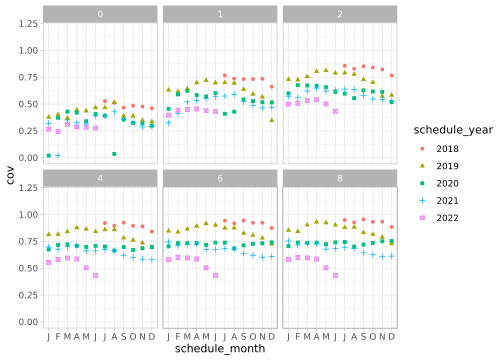
\includegraphics{06_20220405_discussion_files/figure-latex/unnamed-chunk-35-1.pdf}

Aggregate by province

\begin{Shaded}
\begin{Highlighting}[]
\NormalTok{df }\OtherTok{\textless{}{-}}\NormalTok{ measles\_2shots[, }\FunctionTok{c}\NormalTok{(}\StringTok{"pid"}\NormalTok{, }\StringTok{"province"}\NormalTok{, }\StringTok{"vacdate\_1st"}\NormalTok{, }\StringTok{"vtimes"}\NormalTok{,}
    \StringTok{"type2"}\NormalTok{)]}
\NormalTok{df }\OtherTok{\textless{}{-}}\NormalTok{ df }\SpecialCharTok{\%\textgreater{}\%}
    \FunctionTok{pivot\_wider}\NormalTok{(., }\AttributeTok{names\_from =}\NormalTok{ vtimes, }\AttributeTok{values\_from =}\NormalTok{ type2)}

\NormalTok{df}\SpecialCharTok{$}\NormalTok{vyear\_1st }\OtherTok{\textless{}{-}} \FunctionTok{year}\NormalTok{(df}\SpecialCharTok{$}\NormalTok{vacdate\_1st)}
\NormalTok{df}\SpecialCharTok{$}\NormalTok{vmonth\_1st }\OtherTok{\textless{}{-}} \FunctionTok{month}\NormalTok{(df}\SpecialCharTok{$}\NormalTok{vacdate\_1st)}

\NormalTok{df\_type }\OtherTok{\textless{}{-}} \FunctionTok{aggregate}\NormalTok{(pid }\SpecialCharTok{\textasciitilde{}}\NormalTok{ vyear\_1st }\SpecialCharTok{+}\NormalTok{ vmonth\_1st }\SpecialCharTok{+}\NormalTok{ province }\SpecialCharTok{+}
\NormalTok{    shot1 }\SpecialCharTok{+}\NormalTok{ shot2, }\AttributeTok{data =}\NormalTok{ df, }\AttributeTok{FUN =}\NormalTok{ length)}

\NormalTok{df\_type }\OtherTok{\textless{}{-}}\NormalTok{ df\_type }\SpecialCharTok{\%\textgreater{}\%}
    \FunctionTok{group\_by}\NormalTok{(vyear\_1st, province, vmonth\_1st, shot1) }\SpecialCharTok{\%\textgreater{}\%}
    \FunctionTok{mutate}\NormalTok{(}\AttributeTok{denom =} \FunctionTok{sum}\NormalTok{(pid))}

\NormalTok{df\_type}\SpecialCharTok{$}\NormalTok{pct2 }\OtherTok{\textless{}{-}} \DecValTok{100} \SpecialCharTok{*}\NormalTok{ df\_type}\SpecialCharTok{$}\NormalTok{pid}\SpecialCharTok{/}\NormalTok{df\_type}\SpecialCharTok{$}\NormalTok{denom}

\CommentTok{\# An example}
\NormalTok{df\_type }\SpecialCharTok{\%\textgreater{}\%}
    \FunctionTok{filter}\NormalTok{(vyear\_1st }\SpecialCharTok{==} \DecValTok{2018} \SpecialCharTok{\&}\NormalTok{ province }\SpecialCharTok{==} \StringTok{"Ha Noi"} \SpecialCharTok{\&}\NormalTok{ vmonth\_1st }\SpecialCharTok{==}
        \DecValTok{1}\NormalTok{) }\SpecialCharTok{\%\textgreater{}\%}
    \FunctionTok{print}\NormalTok{()}
\end{Highlighting}
\end{Shaded}

\begin{verbatim}
## # A tibble: 4 x 8
## # Groups:   vyear_1st, province, vmonth_1st, shot1 [2]
##   vyear_1st vmonth_1st province shot1   shot2     pid denom  pct2
##       <dbl>      <dbl> <chr>    <fct>   <fct>   <int> <int> <dbl>
## 1      2018          1 Ha Noi   private private   281   702  40.0
## 2      2018          1 Ha Noi   public  private  2852  8192  34.8
## 3      2018          1 Ha Noi   private public    421   702  60.0
## 4      2018          1 Ha Noi   public  public   5340  8192  65.2
\end{verbatim}

Plot by province

\begin{Shaded}
\begin{Highlighting}[]
\CommentTok{\# Get only row that 2nd shot is private}
\NormalTok{df\_plot }\OtherTok{\textless{}{-}}\NormalTok{ df\_type[df\_type}\SpecialCharTok{$}\NormalTok{shot2 }\SpecialCharTok{==} \StringTok{"private"}\NormalTok{, ]}

\CommentTok{\# To plot on a date format x{-}axis}
\NormalTok{df\_plot}\SpecialCharTok{$}\NormalTok{vacdate\_1st }\OtherTok{\textless{}{-}} \FunctionTok{ym}\NormalTok{(}\FunctionTok{paste0}\NormalTok{(df\_plot}\SpecialCharTok{$}\NormalTok{vyear\_1st, }\StringTok{"{-}"}\NormalTok{, df\_plot}\SpecialCharTok{$}\NormalTok{vmonth\_1st))}

\CommentTok{\# Subset from 09/2017 to 03/2020}
\NormalTok{df\_plot }\OtherTok{\textless{}{-}}\NormalTok{ df\_plot[df\_plot}\SpecialCharTok{$}\NormalTok{vacdate\_1st }\SpecialCharTok{\textgreater{}=} \StringTok{"2017{-}09{-}01"} \SpecialCharTok{\&}\NormalTok{ df\_plot}\SpecialCharTok{$}\NormalTok{vacdate\_1st }\SpecialCharTok{\textless{}=}
    \StringTok{"2020{-}03{-}01"}\NormalTok{, ]}

\NormalTok{df\_plot}\SpecialCharTok{$}\NormalTok{shot1 }\OtherTok{\textless{}{-}} \FunctionTok{factor}\NormalTok{(df\_plot}\SpecialCharTok{$}\NormalTok{shot1, }\AttributeTok{levels =} \FunctionTok{c}\NormalTok{(}\StringTok{"public"}\NormalTok{, }\StringTok{"private"}\NormalTok{))}

\FunctionTok{ggplot}\NormalTok{(df\_plot, }\FunctionTok{aes}\NormalTok{(}\AttributeTok{x =}\NormalTok{ vacdate\_1st, }\AttributeTok{y =}\NormalTok{ pct2, }\AttributeTok{group =}\NormalTok{ shot1)) }\SpecialCharTok{+}
    \FunctionTok{geom\_line}\NormalTok{(}\FunctionTok{aes}\NormalTok{(}\AttributeTok{linetype =}\NormalTok{ shot1), }\AttributeTok{stat =} \StringTok{"identity"}\NormalTok{) }\SpecialCharTok{+} \FunctionTok{geom\_vline}\NormalTok{(}\AttributeTok{xintercept =} \FunctionTok{as.numeric}\NormalTok{(}\FunctionTok{as.Date}\NormalTok{(}\StringTok{"2019{-}07{-}01"}\NormalTok{)),}
    \AttributeTok{color =} \StringTok{"orange"}\NormalTok{) }\SpecialCharTok{+} \FunctionTok{facet\_wrap}\NormalTok{(. }\SpecialCharTok{\textasciitilde{}}\NormalTok{ province) }\SpecialCharTok{+} \FunctionTok{ylim}\NormalTok{(}\FunctionTok{c}\NormalTok{(}\DecValTok{0}\NormalTok{,}
    \DecValTok{100}\NormalTok{)) }\SpecialCharTok{+} \FunctionTok{theme\_minimal}\NormalTok{() }\SpecialCharTok{+} \FunctionTok{labs}\NormalTok{(}\AttributeTok{x =} \StringTok{"Month of receiving 1st dose"}\NormalTok{,}
    \AttributeTok{y =} \StringTok{"\% 2nd dose in private"}\NormalTok{, }\AttributeTok{linetype =} \StringTok{"1st dose in"}\NormalTok{) }\SpecialCharTok{+}
    \FunctionTok{theme}\NormalTok{(}\AttributeTok{axis.text.x =} \FunctionTok{element\_blank}\NormalTok{(), }\AttributeTok{panel.grid.minor.x =} \FunctionTok{element\_blank}\NormalTok{())}
\end{Highlighting}
\end{Shaded}

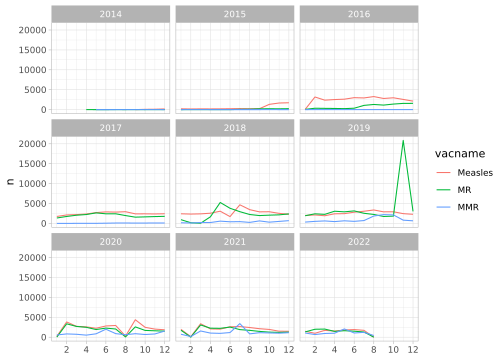
\includegraphics{06_20220405_discussion_files/figure-latex/unnamed-chunk-37-1.pdf}

\hypertarget{population-level}{%
\subsection{Population level}\label{population-level}}

\begin{Shaded}
\begin{Highlighting}[]
\NormalTok{df }\OtherTok{\textless{}{-}}\NormalTok{ measle\_all[, }\FunctionTok{c}\NormalTok{(}\StringTok{"pid"}\NormalTok{, }\StringTok{"province"}\NormalTok{, }\StringTok{"vyear"}\NormalTok{, }\StringTok{"vmonth"}\NormalTok{, }\StringTok{"type2"}\NormalTok{)]}
\NormalTok{df\_type }\OtherTok{\textless{}{-}} \FunctionTok{aggregate}\NormalTok{(pid }\SpecialCharTok{\textasciitilde{}}\NormalTok{ vyear }\SpecialCharTok{+}\NormalTok{ vmonth }\SpecialCharTok{+}\NormalTok{ type2, }\AttributeTok{data =}\NormalTok{ df,}
    \AttributeTok{FUN =}\NormalTok{ length)}

\CommentTok{\# Percentage of private}
\NormalTok{df\_type }\OtherTok{\textless{}{-}}\NormalTok{ df\_type }\SpecialCharTok{\%\textgreater{}\%}
    \FunctionTok{group\_by}\NormalTok{(vyear, vmonth) }\SpecialCharTok{\%\textgreater{}\%}
    \FunctionTok{mutate}\NormalTok{(}\AttributeTok{denom =} \FunctionTok{sum}\NormalTok{(pid))}

\NormalTok{df\_type}\SpecialCharTok{$}\NormalTok{pct }\OtherTok{\textless{}{-}} \DecValTok{100} \SpecialCharTok{*}\NormalTok{ df\_type}\SpecialCharTok{$}\NormalTok{pid}\SpecialCharTok{/}\NormalTok{df\_type}\SpecialCharTok{$}\NormalTok{denom}

\CommentTok{\# Get only row that 2nd shot is private}
\NormalTok{df\_plot }\OtherTok{\textless{}{-}}\NormalTok{ df\_type[df\_type}\SpecialCharTok{$}\NormalTok{type2 }\SpecialCharTok{==} \StringTok{"private"}\NormalTok{, ]}

\CommentTok{\# To plot on a date format x{-}axis}
\NormalTok{df\_plot}\SpecialCharTok{$}\NormalTok{vacdate }\OtherTok{\textless{}{-}} \FunctionTok{ym}\NormalTok{(}\FunctionTok{paste0}\NormalTok{(df\_plot}\SpecialCharTok{$}\NormalTok{vyear, }\StringTok{"{-}"}\NormalTok{, df\_plot}\SpecialCharTok{$}\NormalTok{vmonth))}
\NormalTok{df\_plot }\OtherTok{\textless{}{-}}\NormalTok{ df\_plot[df\_plot}\SpecialCharTok{$}\NormalTok{vacdate }\SpecialCharTok{\textgreater{}=} \StringTok{"2017{-}09{-}01"}\NormalTok{, ]}

\FunctionTok{ggplot}\NormalTok{(df\_plot, }\FunctionTok{aes}\NormalTok{(}\AttributeTok{x =}\NormalTok{ vacdate, }\AttributeTok{y =}\NormalTok{ pct)) }\SpecialCharTok{+} \FunctionTok{geom\_line}\NormalTok{(}\AttributeTok{stat =} \StringTok{"identity"}\NormalTok{) }\SpecialCharTok{+}
    \FunctionTok{geom\_vline}\NormalTok{(}\AttributeTok{xintercept =} \FunctionTok{as.numeric}\NormalTok{(}\FunctionTok{as.Date}\NormalTok{(}\StringTok{"2020{-}04{-}01"}\NormalTok{)),}
        \AttributeTok{color =} \StringTok{"orange"}\NormalTok{) }\SpecialCharTok{+} \FunctionTok{labs}\NormalTok{(}\AttributeTok{y =} \StringTok{"Percentage of private shot"}\NormalTok{,}
    \AttributeTok{x =} \StringTok{"Month of receiving shot"}\NormalTok{) }\SpecialCharTok{+} \FunctionTok{theme\_minimal}\NormalTok{()}
\end{Highlighting}
\end{Shaded}

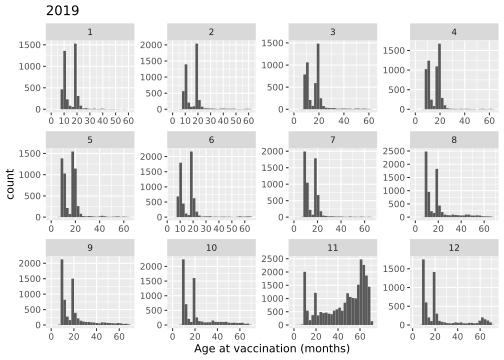
\includegraphics{06_20220405_discussion_files/figure-latex/unnamed-chunk-38-1.pdf}

A sudden increase in percentage of private shot in April because there
were less shots in public (the denominator is low)

\begin{Shaded}
\begin{Highlighting}[]
\NormalTok{df\_plot }\OtherTok{\textless{}{-}} \FunctionTok{data.frame}\NormalTok{(df\_plot)}
\NormalTok{df\_plot[}\FunctionTok{order}\NormalTok{(df\_plot}\SpecialCharTok{$}\NormalTok{vacdate), ]}
\end{Highlighting}
\end{Shaded}

\begin{verbatim}
##    vyear vmonth   type2   pid  denom       pct    vacdate
## 25  2017      9 private    36    474  7.594937 2017-09-01
## 29  2017     10 private   772  22505  3.430349 2017-10-01
## 33  2017     11 private  1790  52177  3.430630 2017-11-01
## 37  2017     12 private  1828  55225  3.310095 2017-12-01
## 1   2018      1 private  2683  56231  4.771389 2018-01-01
## 4   2018      2 private  2244  45005  4.986113 2018-02-01
## 7   2018      3 private  5375  68759  7.817158 2018-03-01
## 10  2018      4 private  5203  63080  8.248256 2018-04-01
## 13  2018      5 private  6527  76754  8.503791 2018-05-01
## 16  2018      6 private  7089  77318  9.168628 2018-06-01
## 19  2018      7 private  9075 113127  8.021958 2018-07-01
## 22  2018      8 private 10925 132428  8.249766 2018-08-01
## 26  2018      9 private 10227 112362  9.101832 2018-09-01
## 30  2018     10 private 11871 118028 10.057783 2018-10-01
## 34  2018     11 private 10649 119010  8.947988 2018-11-01
## 38  2018     12 private 10355 167894  6.167582 2018-12-01
## 2   2019      1 private 11308  98387 11.493388 2019-01-01
## 5   2019      2 private 10439  83395 12.517537 2019-02-01
## 8   2019      3 private 17204 120072 14.328070 2019-03-01
## 11  2019      4 private 15582 113395 13.741347 2019-04-01
## 14  2019      5 private 17836 127113 14.031610 2019-05-01
## 17  2019      6 private 18360 140843 13.035792 2019-06-01
## 20  2019      7 private 19348 139661 13.853545 2019-07-01
## 23  2019      8 private 20662 133728 15.450766 2019-08-01
## 27  2019      9 private 19362 122779 15.769798 2019-09-01
## 31  2019     10 private 21356 127627 16.733136 2019-10-01
## 35  2019     11 private 21800 124771 17.472009 2019-11-01
## 39  2019     12 private 21470 117455 18.279341 2019-12-01
## 3   2020      1 private 18131  87731 20.666583 2020-01-01
## 6   2020      2 private 22358 127126 17.587276 2020-02-01
## 9   2020      3 private 20695 125450 16.496612 2020-03-01
## 12  2020      4 private 15097  52442 28.787994 2020-04-01
## 15  2020      5 private 36325 184711 19.665856 2020-05-01
## 18  2020      6 private 31839 149030 21.364155 2020-06-01
## 21  2020      7 private 33947 144345 23.517960 2020-07-01
## 24  2020      8 private 32955 159425 20.671162 2020-08-01
## 28  2020      9 private 28295 133579 21.182222 2020-09-01
## 32  2020     10 private 24356 106421 22.886460 2020-10-01
## 36  2020     11 private 27443 108791 25.225432 2020-11-01
## 40  2020     12 private 26235 103643 25.312853 2020-12-01
\end{verbatim}

\hypertarget{plot-per-province}{%
\subsection{Plot per province}\label{plot-per-province}}

\begin{Shaded}
\begin{Highlighting}[]
\NormalTok{df\_type }\OtherTok{\textless{}{-}} \FunctionTok{aggregate}\NormalTok{(pid }\SpecialCharTok{\textasciitilde{}}\NormalTok{ vyear }\SpecialCharTok{+}\NormalTok{ province }\SpecialCharTok{+}\NormalTok{ vmonth }\SpecialCharTok{+}\NormalTok{ type2,}
    \AttributeTok{data =}\NormalTok{ df, }\AttributeTok{FUN =}\NormalTok{ length)}

\CommentTok{\# Percentage of private}
\NormalTok{df\_type }\OtherTok{\textless{}{-}}\NormalTok{ df\_type }\SpecialCharTok{\%\textgreater{}\%}
    \FunctionTok{group\_by}\NormalTok{(vyear, province, vmonth) }\SpecialCharTok{\%\textgreater{}\%}
    \FunctionTok{mutate}\NormalTok{(}\AttributeTok{denom =} \FunctionTok{sum}\NormalTok{(pid))}

\NormalTok{df\_type}\SpecialCharTok{$}\NormalTok{pct }\OtherTok{\textless{}{-}} \DecValTok{100} \SpecialCharTok{*}\NormalTok{ df\_type}\SpecialCharTok{$}\NormalTok{pid}\SpecialCharTok{/}\NormalTok{df\_type}\SpecialCharTok{$}\NormalTok{denom}

\CommentTok{\# Get only row that 2nd shot is private}
\NormalTok{df\_plot }\OtherTok{\textless{}{-}}\NormalTok{ df\_type[df\_type}\SpecialCharTok{$}\NormalTok{type2 }\SpecialCharTok{==} \StringTok{"private"}\NormalTok{, ]}

\CommentTok{\# To plot on a date format x{-}axis}
\NormalTok{df\_plot}\SpecialCharTok{$}\NormalTok{vacdate }\OtherTok{\textless{}{-}} \FunctionTok{ym}\NormalTok{(}\FunctionTok{paste0}\NormalTok{(df\_plot}\SpecialCharTok{$}\NormalTok{vyear, }\StringTok{"{-}"}\NormalTok{, df\_plot}\SpecialCharTok{$}\NormalTok{vmonth))}
\NormalTok{df\_plot }\OtherTok{\textless{}{-}}\NormalTok{ df\_plot[df\_plot}\SpecialCharTok{$}\NormalTok{vacdate }\SpecialCharTok{\textgreater{}=} \StringTok{"2017{-}09{-}01"}\NormalTok{, ]}

\FunctionTok{ggplot}\NormalTok{(df\_plot, }\FunctionTok{aes}\NormalTok{(}\AttributeTok{x =}\NormalTok{ vacdate, }\AttributeTok{y =}\NormalTok{ pct)) }\SpecialCharTok{+} \FunctionTok{geom\_line}\NormalTok{(}\AttributeTok{stat =} \StringTok{"identity"}\NormalTok{) }\SpecialCharTok{+}
    \FunctionTok{geom\_vline}\NormalTok{(}\AttributeTok{xintercept =} \FunctionTok{as.numeric}\NormalTok{(}\FunctionTok{as.Date}\NormalTok{(}\StringTok{"2020{-}04{-}01"}\NormalTok{)),}
        \AttributeTok{color =} \StringTok{"orange"}\NormalTok{) }\SpecialCharTok{+} \FunctionTok{facet\_wrap}\NormalTok{(. }\SpecialCharTok{\textasciitilde{}}\NormalTok{ province) }\SpecialCharTok{+} \FunctionTok{labs}\NormalTok{(}\AttributeTok{x =} \StringTok{"Percentage of private shot"}\NormalTok{,}
    \AttributeTok{y =} \StringTok{"Month of receiving shot"}\NormalTok{) }\SpecialCharTok{+} \FunctionTok{theme\_light}\NormalTok{()}
\end{Highlighting}
\end{Shaded}

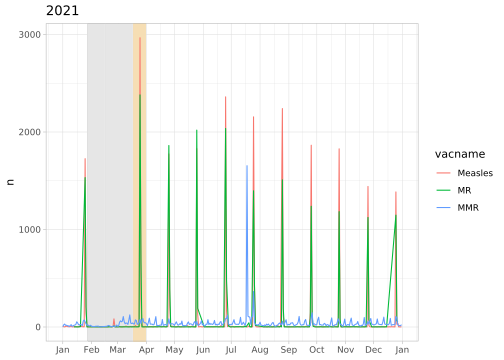
\includegraphics{06_20220405_discussion_files/figure-latex/unnamed-chunk-40-1.pdf}

\hypertarget{missing-measles-shot-for-children-born-in-2019-and-2020-vaccine-measles-at-9-month}{%
\subsection{Missing measles shot for children born in 2019 and 2020:
vaccine Measles (at 9
month)}\label{missing-measles-shot-for-children-born-in-2019-and-2020-vaccine-measles-at-9-month}}

\begin{Shaded}
\begin{Highlighting}[]
\FunctionTok{load}\NormalTok{(}\FunctionTok{file.path}\NormalTok{(allp, }\StringTok{"hepatitisb\_all.Rdata"}\NormalTok{))}

\CommentTok{\# Child in hepB dataset}
\NormalTok{child }\OtherTok{\textless{}{-}}\NormalTok{ hepatitisb\_all[hepatitisb\_all}\SpecialCharTok{$}\NormalTok{province }\SpecialCharTok{\%in\%}\NormalTok{ publicProvinces }\SpecialCharTok{\&}
\NormalTok{    hepatitisb\_all}\SpecialCharTok{$}\NormalTok{year }\SpecialCharTok{==} \DecValTok{2019} \SpecialCharTok{|}\NormalTok{ (hepatitisb\_all}\SpecialCharTok{$}\NormalTok{year }\SpecialCharTok{==} \DecValTok{2020} \SpecialCharTok{\&}
\NormalTok{    hepatitisb\_all}\SpecialCharTok{$}\NormalTok{month }\SpecialCharTok{\textless{}=} \DecValTok{3}\NormalTok{), ]}


\NormalTok{measles\_1920 }\OtherTok{\textless{}{-}}\NormalTok{ measle\_all[measle\_all}\SpecialCharTok{$}\NormalTok{province }\SpecialCharTok{\%in\%}\NormalTok{ publicProvinces }\SpecialCharTok{\&}
\NormalTok{    measle\_all}\SpecialCharTok{$}\NormalTok{year }\SpecialCharTok{==} \DecValTok{2019} \SpecialCharTok{|}\NormalTok{ (measle\_all}\SpecialCharTok{$}\NormalTok{year }\SpecialCharTok{==} \DecValTok{2020} \SpecialCharTok{\&}\NormalTok{ measle\_all}\SpecialCharTok{$}\NormalTok{month }\SpecialCharTok{\textless{}=}
    \DecValTok{3}\NormalTok{), ]}
\NormalTok{id\_measles }\OtherTok{\textless{}{-}} \FunctionTok{unique}\NormalTok{(measles\_1920}\SpecialCharTok{$}\NormalTok{pid)}
\NormalTok{id\_hepb }\OtherTok{\textless{}{-}} \FunctionTok{unique}\NormalTok{(child}\SpecialCharTok{$}\NormalTok{pid[child}\SpecialCharTok{$}\NormalTok{vacname2 }\SpecialCharTok{\%in\%} \FunctionTok{c}\NormalTok{(}\StringTok{"HepB"}\NormalTok{, }\StringTok{"HepBN"}\NormalTok{)])}

\FunctionTok{length}\NormalTok{(}\FunctionTok{intersect}\NormalTok{(id\_measles, id\_hepb))}
\end{Highlighting}
\end{Shaded}

\begin{verbatim}
## [1] 680366
\end{verbatim}

\end{document}
